%%%% ijcai22-multiauthor.tex
%DIF LATEXDIFF DIFFERENCE FILE
%DIF DEL thesis.tex                  Tue Apr 28 19:54:10 2026
%DIF ADD thesis_after_comments.tex   Fri May  8 23:58:16 2026

\typeout{IJCAI--22 Multiple authors example}

% These are the instructions for authors for IJCAI-22.

\documentclass{article}
\pdfpagewidth=8.5in
\pdfpageheight=11in
% The file ijcai22.sty is NOT the same as previous years'
\usepackage{ijcai22}

% Use the postscript times font!
\usepackage{times}
\renewcommand*\ttdefault{txtt}
\usepackage{soul}
\usepackage{url}
\usepackage[hidelinks]{hyperref}
\usepackage[utf8]{inputenc}
\usepackage[small]{caption}
\usepackage{graphicx}
\usepackage{amsmath}
\usepackage{booktabs}
\usepackage{algorithm}
\usepackage{algorithmic}
\urlstyle{same}
\usepackage{xcolor}
\usepackage{multicol}
\usepackage{tikz}

\newcommand\todo[1]{\textcolor{red}{#1}}

% the following package is optional:
%\usepackage{latexsym}

\pdfinfo{
	/TemplateVersion (IJCAI.2022.0)
}


\title{A computational approach for variants of coloring planar graphs}

\author{
	Arne Claerhout$^1$\and
	Jorik Jooken$^1$\And
	Jan Goedgebeur$^1$\\
	\affiliations
	$^1$KU Leuven KULAK
	\emails
	arne.claerhout@student.kuleuven.be,
	jorik.jooken@kuleuven.be,
	jan.goedgebeur@kuleuven.be
}
%DIF PREAMBLE EXTENSION ADDED BY LATEXDIFF
%DIF UNDERLINE PREAMBLE %DIF PREAMBLE
\RequirePackage[normalem]{ulem} %DIF PREAMBLE
\RequirePackage{color}\definecolor{RED}{rgb}{1,0,0}\definecolor{BLUE}{rgb}{0,0,1} %DIF PREAMBLE
\providecommand{\DIFaddtex}[1]{{\protect\color{blue}\uwave{#1}}} %DIF PREAMBLE
\providecommand{\DIFdeltex}[1]{{\protect\color{red}\sout{#1}}}                      %DIF PREAMBLE
%DIF SAFE PREAMBLE %DIF PREAMBLE
\providecommand{\DIFaddbegin}{} %DIF PREAMBLE
\providecommand{\DIFaddend}{} %DIF PREAMBLE
\providecommand{\DIFdelbegin}{} %DIF PREAMBLE
\providecommand{\DIFdelend}{} %DIF PREAMBLE
\providecommand{\DIFmodbegin}{} %DIF PREAMBLE
\providecommand{\DIFmodend}{} %DIF PREAMBLE
%DIF FLOATSAFE PREAMBLE %DIF PREAMBLE
\providecommand{\DIFaddFL}[1]{\DIFadd{#1}} %DIF PREAMBLE
\providecommand{\DIFdelFL}[1]{\DIFdel{#1}} %DIF PREAMBLE
\providecommand{\DIFaddbeginFL}{} %DIF PREAMBLE
\providecommand{\DIFaddendFL}{} %DIF PREAMBLE
\providecommand{\DIFdelbeginFL}{} %DIF PREAMBLE
\providecommand{\DIFdelendFL}{} %DIF PREAMBLE
%DIF HYPERREF PREAMBLE %DIF PREAMBLE
\providecommand{\DIFadd}[1]{\texorpdfstring{\DIFaddtex{#1}}{#1}} %DIF PREAMBLE
\providecommand{\DIFdel}[1]{\texorpdfstring{\DIFdeltex{#1}}{}} %DIF PREAMBLE
\newcommand{\DIFscaledelfig}{0.5}
%DIF HIGHLIGHTGRAPHICS PREAMBLE %DIF PREAMBLE
\RequirePackage{settobox} %DIF PREAMBLE
\RequirePackage{letltxmacro} %DIF PREAMBLE
\newsavebox{\DIFdelgraphicsbox} %DIF PREAMBLE
\newlength{\DIFdelgraphicswidth} %DIF PREAMBLE
\newlength{\DIFdelgraphicsheight} %DIF PREAMBLE
% store original definition of \includegraphics %DIF PREAMBLE
\LetLtxMacro{\DIFOincludegraphics}{\includegraphics} %DIF PREAMBLE
\newcommand{\DIFaddincludegraphics}[2][]{{\color{blue}\fbox{\DIFOincludegraphics[#1]{#2}}}} %DIF PREAMBLE
\newcommand{\DIFdelincludegraphics}[2][]{% %DIF PREAMBLE
\sbox{\DIFdelgraphicsbox}{\DIFOincludegraphics[#1]{#2}}% %DIF PREAMBLE
\settoboxwidth{\DIFdelgraphicswidth}{\DIFdelgraphicsbox} %DIF PREAMBLE
\settoboxtotalheight{\DIFdelgraphicsheight}{\DIFdelgraphicsbox} %DIF PREAMBLE
\scalebox{\DIFscaledelfig}{% %DIF PREAMBLE
\parbox[b]{\DIFdelgraphicswidth}{\usebox{\DIFdelgraphicsbox}\\[-\baselineskip] \rule{\DIFdelgraphicswidth}{0em}}\llap{\resizebox{\DIFdelgraphicswidth}{\DIFdelgraphicsheight}{% %DIF PREAMBLE
\setlength{\unitlength}{\DIFdelgraphicswidth}% %DIF PREAMBLE
\begin{picture}(1,1)% %DIF PREAMBLE
\thicklines\linethickness{2pt} %DIF PREAMBLE
{\color[rgb]{1,0,0}\put(0,0){\framebox(1,1){}}}% %DIF PREAMBLE
{\color[rgb]{1,0,0}\put(0,0){\line( 1,1){1}}}% %DIF PREAMBLE
{\color[rgb]{1,0,0}\put(0,1){\line(1,-1){1}}}% %DIF PREAMBLE
\end{picture}% %DIF PREAMBLE
}\hspace*{3pt}}} %DIF PREAMBLE
} %DIF PREAMBLE
\LetLtxMacro{\DIFOaddbegin}{\DIFaddbegin} %DIF PREAMBLE
\LetLtxMacro{\DIFOaddend}{\DIFaddend} %DIF PREAMBLE
\LetLtxMacro{\DIFOdelbegin}{\DIFdelbegin} %DIF PREAMBLE
\LetLtxMacro{\DIFOdelend}{\DIFdelend} %DIF PREAMBLE
\DeclareRobustCommand{\DIFaddbegin}{\DIFOaddbegin \let\includegraphics\DIFaddincludegraphics} %DIF PREAMBLE
\DeclareRobustCommand{\DIFaddend}{\DIFOaddend \let\includegraphics\DIFOincludegraphics} %DIF PREAMBLE
\DeclareRobustCommand{\DIFdelbegin}{\DIFOdelbegin \let\includegraphics\DIFdelincludegraphics} %DIF PREAMBLE
\DeclareRobustCommand{\DIFdelend}{\DIFOaddend \let\includegraphics\DIFOincludegraphics} %DIF PREAMBLE
\LetLtxMacro{\DIFOaddbeginFL}{\DIFaddbeginFL} %DIF PREAMBLE
\LetLtxMacro{\DIFOaddendFL}{\DIFaddendFL} %DIF PREAMBLE
\LetLtxMacro{\DIFOdelbeginFL}{\DIFdelbeginFL} %DIF PREAMBLE
\LetLtxMacro{\DIFOdelendFL}{\DIFdelendFL} %DIF PREAMBLE
\DeclareRobustCommand{\DIFaddbeginFL}{\DIFOaddbeginFL \let\includegraphics\DIFaddincludegraphics} %DIF PREAMBLE
\DeclareRobustCommand{\DIFaddendFL}{\DIFOaddendFL \let\includegraphics\DIFOincludegraphics} %DIF PREAMBLE
\DeclareRobustCommand{\DIFdelbeginFL}{\DIFOdelbeginFL \let\includegraphics\DIFdelincludegraphics} %DIF PREAMBLE
\DeclareRobustCommand{\DIFdelendFL}{\DIFOaddendFL \let\includegraphics\DIFOincludegraphics} %DIF PREAMBLE
%DIF LISTINGS PREAMBLE %DIF PREAMBLE
\RequirePackage{listings} %DIF PREAMBLE
\RequirePackage{color} %DIF PREAMBLE
\lstdefinelanguage{DIFcode}{ %DIF PREAMBLE
%DIF DIFCODE_UNDERLINE %DIF PREAMBLE
  moredelim=[il][\color{red}\sout]{\%DIF\ <\ }, %DIF PREAMBLE
  moredelim=[il][\color{blue}\uwave]{\%DIF\ >\ } %DIF PREAMBLE
} %DIF PREAMBLE
\lstdefinestyle{DIFverbatimstyle}{ %DIF PREAMBLE
	language=DIFcode, %DIF PREAMBLE
	basicstyle=\ttfamily, %DIF PREAMBLE
	columns=fullflexible, %DIF PREAMBLE
	keepspaces=true %DIF PREAMBLE
} %DIF PREAMBLE
\lstnewenvironment{DIFverbatim}{\lstset{style=DIFverbatimstyle}}{} %DIF PREAMBLE
\lstnewenvironment{DIFverbatim*}{\lstset{style=DIFverbatimstyle,showspaces=true}}{} %DIF PREAMBLE
%DIF END PREAMBLE EXTENSION ADDED BY LATEXDIFF

\begin{document}

\maketitle

\begin{abstract}
	In this paper, \DIFdelbegin \DIFdel{we study the coloring of planar graphs for different variants of graph colorings. In particular, }\DIFdelend \DIFaddbegin \DIFadd{a backtracking algorithm is proposed to color planar graphs according to }\DIFaddend the proper, odd, conflict-free and unique-maximum vertex colorings\DIFdelbegin \DIFdel{are examined. This paper proposes a backtracking algorithm to color planar graphs}\DIFdelend .

	The chromatic numbers of these coloring variants are also studied further. These are the minimum number of colors needed to color any planar graph.
	\DIFdelbegin %DIFDELCMD < 

%DIFDELCMD < 	%%%
\DIFdelend Not all chromatic numbers are known, therefore, conjectures exist. This algorithm can be used to disprove or substantiate these conjectures.

	The \DIFaddbegin \DIFadd{developed }\DIFaddend algorithm was constructed by applying optimizations to a naive algorithm. The final implementation is a fully optimized algorithm implemented in C.

	The proposed algorithm does not outperform alternatives, but is only around $1.4$ times slower \DIFdelbegin \DIFdel{, }\DIFdelend for the proper coloring. The algorithm does have the added benefit of easy expandability for other undiscussed coloring variants. No other \DIFdelbegin \DIFdel{programs }\DIFdelend \DIFaddbegin \DIFadd{tools }\DIFaddend exist for the other coloring variants, therefore, \DIFdelbegin \DIFdel{these }\DIFdelend \DIFaddbegin \DIFadd{this part of the algorithm }\DIFaddend can not be compared.

	It was \DIFdelbegin \DIFdel{also }\DIFdelend found that the conjectures that \DIFdelbegin \DIFdel{haven't }\DIFdelend \DIFaddbegin \DIFadd{have not }\DIFaddend been disproven yet are correct for all planar triangulations with $20$ or less vertices. 

\end{abstract}

\section{Introduction}

Graph theory is a field of research in computer science that is older than the computer. Its conception dating back to the 18th century \cite{euler1741solutio}. 

A \textit{graph} $G = (V, E)$ is defined as a pair, containing a collection of vertices ($V$) and edges ($E$). Each edge is an unordered pair of unique vertices. A \textit{planar graph} is a variant of graphs such that a planar embedding is possible without edges crossing. Planar graphs and graphs will be used interchangeably. The \textit{class of planar graphs} $\mathcal{P}$ is defined as the set of all planar graphs. \textit{Planar triangulations}, a subset of planar graphs, are graphs with the maximum number of edges for some number of vertices, this means the addition of an edge would break the planarity of the graph.

The coloring of graphs is one of the most well-known fields in graph theory. A coloring of a graph is a function assigning each vertex a color $1, \dots, k$. The most famous of these colorings is the\DIFdelbegin \DIFdel{proper coloring}\DIFdelend \DIFaddbegin \textit{ \DIFadd{proper coloring}}\DIFaddend . This states that two \DIFdelbegin \DIFdel{adjacent vertices---vertices sharing an edge---never }\DIFdelend \DIFaddbegin \DIFadd{vertices sharing an edge, never }\DIFaddend share the same color. 

The \DIFdelbegin \DIFdel{chromatic number }\DIFdelend \DIFaddbegin \textit{\DIFadd{chromatic number}} \DIFaddend $\chi(G)$ of a graph $G$ is the minimum number of colors needed to color \DIFdelbegin \DIFdel{the }\DIFdelend \DIFaddbegin \DIFadd{that }\DIFaddend graph. A generalization of this is the chromatic number $\chi(\mathcal{P})$ for the class of planar graphs, which is the minimum number of needed colors to color \textit{any} planar graph. For the proper coloring, it was proven that four colors always suffice \cite{appel1976every}. This was a special result, as this was the first \DIFaddbegin \DIFadd{ever }\DIFaddend proof verified using a computer program.

Coloring of graphs has various applications, with uses including: the assignment of frequencies to radio stations, the coloring of maps, scheduling and more.

There exist many variants of graph colorings. One such variant is an \textit{odd coloring}, which was recently introduced by Petruševski and Škrekovski \DIFdelbegin \DIFdel{\mbox{%DIFAUXCMD
\cite{PETRUSEVSKI2022385} }\hspace{0pt}%DIFAUXCMD
}\DIFdelend in $2022$ \DIFaddbegin \DIFadd{\mbox{%DIFAUXCMD
\cite{PETRUSEVSKI2022385}}\hspace{0pt}%DIFAUXCMD
}\DIFaddend . A proper coloring of a graph is said to be odd if \DIFdelbegin \DIFdel{for }\DIFdelend each vertex $v \in V$ \DIFdelbegin \DIFdel{there exists a }\DIFdelend \DIFaddbegin \DIFadd{has at least one }\DIFaddend color occurring an odd \DIFdelbegin \DIFdel{amount }\DIFdelend \DIFaddbegin \DIFadd{number }\DIFaddend of times in \DIFdelbegin \DIFdel{the neighborhood of that vertex }\DIFdelend \DIFaddbegin \DIFadd{its neighborhood }\DIFaddend $N(v)$. The \textit{odd chromatic number} $\chi_{\mathrm{O}}(\mathcal{P})$ is the minimal number of colors needed to color any \DIFaddbegin \DIFadd{planar }\DIFaddend graph with an odd coloring.

\DIFdelbegin \DIFdel{The other variants are }\DIFdelend \DIFaddbegin \DIFadd{Other variants include }\DIFaddend conflict-free and unique-maximum colorings. 

The \textit{conflict-free coloring}, introduced in 2003 by Even, Lotker, Ron, and Smorodinsky \cite{even2003conflict}, is a coloring such that every vertex has at least one unique color in its neighborhood\DIFdelbegin \DIFdel{. This is }\DIFdelend \DIFaddbegin \DIFadd{, }\DIFaddend useful because of applications in wireless networks and more \cite{smorodinsky2013conflict}.

\DIFdelbegin \DIFdel{Now consider a }\textit{\DIFdel{proper conflict-free coloring}} %DIFAUXCMD
\DIFdel{with respect to open- or closed neighborhoods---a conflict-free coloringwith an added proper constraint. The conflict-free property is tested on the open- or closed neighborhood of vertices . 
An open neighborhood }\DIFdelend \DIFaddbegin \DIFadd{To distinguish between different versions of this coloring, neighborhoods of vertices must be defined. An }\textit{\DIFadd{open neighborhood}} \DIFaddend of a vertex $v$ is defined as $N(v) = \{w | (v, w) \in E\}$\DIFdelbegin \DIFdel{. This does therefore not include }\DIFdelend \DIFaddbegin \DIFadd{: containing all vertices sharing an edge with $v$, therefore not including }\DIFaddend the vertex $v$ itself. A \DIFdelbegin \DIFdel{closed neighborhood }\DIFdelend \DIFaddbegin \textit{\DIFadd{closed neighborhood}} \DIFaddend of a vertex $v$ is $N[v] = N(v) \cup \{v\}$\DIFdelbegin \DIFdel{, }\DIFdelend \DIFaddbegin \DIFadd{: }\DIFaddend the open neighborhood of $v$, including the vertex itself. 
\DIFdelbegin \DIFdel{Both colorings }\DIFdelend \DIFaddbegin 

\DIFadd{Now consider }\textit{\DIFadd{proper conflict-free colorings}} \DIFadd{with respect to open- or closed neighborhoods: a conflict-free coloring where all neighboring vertices have different colors. Depending on which neighborhood definition is used
Both }\DIFaddend have \textit{chromatic numbers} $\chi_{\mathrm{pCFo}}(\mathcal{P})$ and $\chi_{\mathrm{pCFc}}(\mathcal{P})$ respectively, with the $o$ and $c$ signaling open- or closed neighborhoods.


Similarly, \DIFdelbegin \DIFdel{an }\DIFdelend \textit{improper conflict-free \DIFdelbegin \DIFdel{coloring}\DIFdelend \DIFaddbegin \DIFadd{colorings}\DIFaddend } with respect to open- or closed neighborhoods can be defined\DIFdelbegin \DIFdel{. These are the same colorings, }\DIFdelend \DIFaddbegin \DIFadd{, the same coloring versions as before, but }\DIFaddend without the proper constraint. Again, \DIFaddbegin \DIFadd{both coloring versions have respective }\DIFaddend \textit{chromatic numbers} $\chi_{\mathrm{iCFo}}(\mathcal{P})$ and $\chi_{\mathrm{iCFc}}(\mathcal{P})$\DIFdelbegin \DIFdel{respectively can be defined for both}\DIFdelend .

\textit{Unique-maximum colorings} stem from ordered colorings \cite{KATCHALSKI1995141}, and were studied further in the context of open- and closed neighborhoods by Fabrici, Lužar, Rindošová and Soták \cite{fabrici2023proper}. This is a coloring where the maximum color appearing in the neighborhood of a vertex appears exactly once in \DIFdelbegin \DIFdel{the neighborhoodof that vertex}\DIFdelend \DIFaddbegin \DIFadd{its neighborhood}\DIFaddend .

Using the same splitting as the conflict-free coloring, four versions of this coloring can be defined\DIFdelbegin \DIFdel{. A }\DIFdelend \DIFaddbegin \DIFadd{: }\DIFaddend proper unique-maximum \DIFdelbegin \DIFdel{coloring }\DIFdelend \DIFaddbegin \DIFadd{colorings }\DIFaddend with respect to open- or closed neighborhoods, and \DIFdelbegin \DIFdel{an }\DIFdelend improper unique-maximum \DIFdelbegin \DIFdel{coloring }\DIFdelend \DIFaddbegin \DIFadd{colorings }\DIFaddend with respect to open- or closed neighborhoods. Each respectively having their own \textit{chromatic number} for the class of planar graphs: $\chi_{\mathrm{pUMo}}(\mathcal{P})$, $\chi_{\mathrm{pUMc}}(\mathcal{P})$, $\chi_{\mathrm{iUMo}}(\mathcal{P})$ and $\chi_{\mathrm{iUMc}}(\mathcal{P})$.

\subsection{Known bounds}
\DIFaddbegin \label{sec:bounds}
\DIFaddend 

Not all chromatic numbers of these \DIFdelbegin \DIFdel{colorings }\DIFdelend \DIFaddbegin \DIFadd{coloring variants }\DIFaddend are known. For most, only bounds exist, where some upper bound always suffices to color \DIFdelbegin \DIFdel{all }\DIFdelend \DIFaddbegin \textit{\DIFadd{all}} \DIFadd{planar }\DIFaddend graphs, while the lower bound is derived from a graph with the highest \textit{found} chromatic number. 

As the unique color for each vertex $v$ in the $\mathrm{pCFc}$-coloring can always be the color of $v$ itself, this coloring is exactly equal to the proper coloring. Therefore, $\chi_{\mathrm{pCFc}}(\mathcal{P})$ is equal to $4$, \DIFdelbegin \DIFdel{just like }\DIFdelend \DIFaddbegin \DIFadd{the same as }\DIFaddend the chromatic number of the proper coloring.

The bounds for all \DIFdelbegin \DIFdel{colorings }\DIFdelend \DIFaddbegin \DIFadd{coloring variants }\DIFaddend are as follows:


\begin{itemize}
	\item The odd coloring:
	\begin{itemize}
		\item $5 \leq \chi_{\mathrm{O}}(\mathcal{P}) \leq 8$ (\textit{proven by \cite{petr2023odd} for upper bound, lower bound is $\mathit{C_5}$\DIFaddbegin \DIFadd{: cycle of length $5$}\DIFaddend })
	\end{itemize}

	\item \DIFdelbegin \DIFdel{the }\DIFdelend \DIFaddbegin \DIFadd{The }\DIFaddend conflict-free colorings:
	\begin{itemize}
		\item $6 \leq \chi_{\mathrm{pCFo}}(\mathcal{P}) \leq 8$ (\textit{proven by \cite{fabrici2023proper}})
		\item $\chi_{\mathrm{pCFc}}(\mathcal{P}) = 4$ \DIFaddbegin \DIFadd{(}\textit{\DIFadd{proven by \mbox{%DIFAUXCMD
\cite{appel1976every}}\hspace{0pt}%DIFAUXCMD
}}\DIFadd{)
		}\DIFaddend \item $4 \le \chi_{\mathrm{iCFo}}(\mathcal{P}) \le 5$ (\textit{proven by \cite{abel2018conflict} for lower bound and \cite{huang2020short} for upper bound})
		\item $\chi_{\mathrm{iCFc}}(\mathcal{P}) = 4$ (\textit{proven by \cite{Malik2023thesis} \DIFaddbegin \DIFadd{for lower bound and upper bound is $\mathit{\chi_{\mathrm{pCFc}}(\mathcal{P})}$ because proper coloring is invariably improper}\DIFaddend })
	\end{itemize}

	\item The unique-maximum colorings (all \textit{proven by \cite{fabrici2023proper}}):
	\begin{itemize}
		\item $6 \leq \chi_{\mathrm{pUMo}}(\mathcal{P}) \leq 10$
		\item $6 \leq \chi_{\mathrm{pUMc}}(\mathcal{P}) \leq 8$
		\item $5 \le \chi_{\mathrm{iUMo}}(\mathcal{P}) \le 10$
		\item $4 \le \chi_{\mathrm{iUMc}}(\mathcal{P}) \le 6$
	\end{itemize}
\end{itemize}



\subsection{Conjectures}
\label{sect:Conjectures}

As most of the chromatic numbers are not known. Some authors started formulating conjectures on this problem.

Petruševski and Škrekovski, the originators of the odd coloring, conjectured $\chi_{\mathrm{O}}(\mathcal{P}) = 5$. Other conjectures introduced by Fabrici, Lužar, Rindošová and Soták \cite{fabrici2023proper} include:

\begin{minipage}{0.45\textwidth}
	\raggedcolumns
	\begin{multicols}{2}
		\begin{itemize}
			\item $\chi_{\mathrm{pUMo}}(\mathcal{P}) \leq 7$
			\item $\chi_{\mathrm{pUMc}}(\mathcal{P}) = 6$
			\item $\chi_{\mathrm{iUMo}}(\mathcal{P}) = 5$
			\item $\chi_{\mathrm{iUMc}}(\mathcal{P}) = 4$
			\item $\chi_{\mathrm{pCFo}}(\mathcal{P}) = 6$
			\item $\chi_{\mathrm{iCFo}}(\mathcal{P}) = 4$
			\item $\chi_{\mathrm{iCFc}}(\mathcal{P}) = 3$
		\end{itemize}
	\end{multicols}
\end{minipage}
\vspace{0.4cm}

Since then, the conjecture for the chromatic number of the $\mathrm{iCFc}$-coloring has been disproven\DIFaddbegin \DIFadd{, with the exact chromatic number now being known, as shown in Section \ref{sec:bounds}}\DIFaddend .


\subsection{Research Problem}

In this paper, two research questions are considered:

\begin{itemize}
	\item \textbf{Can we design an algorithm for coloring planar graphs, faster than or just as fast as the existing coloring algorithms, that is also easily expandable to new coloring variants?}
	\item \textbf{In what way is this algorithm useful in helping to prove or disprove conjectures surrounding these coloring variants?}
\end{itemize}

The focus is mostly laid on the \DIFdelbegin \DIFdel{designing }\DIFdelend \DIFaddbegin \DIFadd{design process }\DIFaddend of the mentioned algorithm. Further results are also discussed.

The structure of this paper is as follows. First, the algorithm developed is discussed in Section \ref{sec:alg} by examining the the \DIFdelbegin \DIFdel{pseudo-code}\DIFdelend \DIFaddbegin \DIFadd{pseudocode}\DIFaddend . Afterwards, the implementation of said algorithm is discussed in Section \ref{sec:implementation}. Here, all notable optimizations applied are studied further. Then, the results of this paper are discussed further in Section \ref{sec:results}. Lastly, the threats to validity are discussed in Section \ref{sec:threats}, ending with the conclusion in Section \ref{sec:conclusion}.


\section{Algorithm}
\label{sec:alg}

In this section\DIFdelbegin \DIFdel{the developed }\DIFdelend \DIFaddbegin \DIFadd{, the developed backtracking }\DIFaddend algorithm is discussed\DIFdelbegin \DIFdel{. A backtracking algorithm was used, coloring the vertices }\DIFdelend \DIFaddbegin \DIFadd{, where the vertices are colored }\DIFaddend one-by-one and pruning \DIFaddbegin \DIFadd{is utilized }\DIFaddend where possible. The \DIFdelbegin \DIFdel{pseudo-code is found }\DIFdelend \DIFaddbegin \DIFadd{pseudocode is displayed }\DIFaddend in Algorithms \ref{alg:search}, \ref{alg:check}, \ref{alg:updateN} and \ref{alg:special}. 


\DIFdelbegin \DIFdel{Starting with }\DIFdelend \DIFaddbegin \DIFadd{We start by explaining }\DIFaddend Algorithm \ref{alg:search}, \DIFdelbegin \DIFdel{this is }\DIFdelend the `overseer' of the \DIFdelbegin \DIFdel{algorithm. Only choosing }\DIFdelend \DIFaddbegin \DIFadd{entire algorithm. It only chooses }\DIFaddend a maximum color \DIFaddbegin \DIFadd{$max\_c$ }\DIFaddend for the graph and \DIFdelbegin \DIFdel{letting }\DIFdelend \DIFaddbegin \DIFadd{lets }\DIFaddend the recursive algorithm check if the coloring is possible for that maximum. This is also reflected in the \DIFdelbegin \DIFdel{pseudo-code. 
}%DIFDELCMD < 

%DIFDELCMD < %%%
\DIFdel{Before checking the }\DIFdelend \DIFaddbegin \DIFadd{pseudocode. 
Before checking this }\DIFaddend maximum color, the available colors of the vertices are reset to reflect \DIFdelbegin \DIFdel{the maximum color (}\DIFdelend \DIFaddbegin \DIFadd{$max\_c$ (}\DIFaddend \textit{e.g., if the maximum color is \DIFdelbegin \DIFdel{3}\DIFdelend \DIFaddbegin \DIFadd{$3$}\DIFaddend , the available colors \DIFdelbegin \DIFdel{are }\DIFdelend \DIFaddbegin \DIFadd{will be }\DIFaddend ${1, 2 \text{ and } 3}$})\DIFaddbegin \DIFadd{, as this will be used for early pruning}\DIFaddend .

Algorithm \ref{alg:check} is the main checking \DIFaddbegin \DIFadd{component of the }\DIFaddend algorithm. It checks whether the given graph $G$ can be colored given a maximum color $max\_c$. This is done in multiple steps, starting with a base case: if all vertices are colored, a valid coloring is reached, which \DIFdelbegin \DIFdel{notifies the previous recursion step}\DIFdelend \DIFaddbegin \DIFadd{means the chromatic number is found for the graph $G$}\DIFaddend . 

Otherwise, it loops over all available colors of the given vertex\DIFdelbegin \DIFdel{, where }\DIFdelend \DIFaddbegin \DIFadd{. Here, }\DIFaddend permutations are avoided\DIFdelbegin \DIFdel{. This means it will check if that available color is one higher or less }\DIFdelend \DIFaddbegin \DIFadd{, meaning the algorithm makes sure the new color is maximally one higher }\DIFaddend than the current maximum color in the graph. \DIFdelbegin \DIFdel{If so, a lower color should be assigned and this available color should get skipped. }\DIFdelend This optimization is further \DIFaddbegin \DIFadd{explained and }\DIFaddend discussed in Section \ref{sec:optim}.

Next, the $vertex$ is colored with \DIFdelbegin \DIFdel{the }\DIFdelend \DIFaddbegin \DIFadd{an }\DIFaddend available color $c$\DIFdelbegin \DIFdel{, and all neighbors of that }\DIFdelend \DIFaddbegin \DIFadd{. 
Afterwards, the neighbors of }\DIFaddend $vertex$ are updated\DIFdelbegin \DIFdel{using the }\texttt{\DIFdel{update\_neighbors}} %DIFAUXCMD
\DIFdel{function. This will essentially update the available colors of all neighbors and those neighbors' neighbors, and check if the coloring is still possible. If not, the progress made this recursion step is reset, and the next available color is tried. If the coloring is }\textit{\DIFdel{still}} %DIFAUXCMD
\DIFdel{possible, the next recursion step is called with a new $index$ and $depth$}\DIFdelend . \DIFdelbegin %DIFDELCMD < 

%DIFDELCMD < %%%
\DIFdel{The }\texttt{\DIFdel{update\_neighbors}} %DIFAUXCMD
\DIFdel{function is therefore the function checking the correctness of the coloring. If the coloring isn't valid, the graph goes back a recursion step, therefore backtracking. All checks are done while the algorithm is coloring, which is the reason the base case does not check this anymore.
}%DIFDELCMD < 

%DIFDELCMD < %%%
\DIFdel{After trying all available colors without results, the vertex color is reset and the previous recursion step is notified of failure.
}%DIFDELCMD < 

%DIFDELCMD < %%%
\DIFdel{The $depth$ variable is used in the }\texttt{\DIFdel{add\_colors\_back}} %DIFAUXCMD
\DIFdel{function. All of the changes in the entire algorithm, meaning all updates for all vertices and all recursion steps, are kept track of. The $depth$ is used to log changes and restore them.
}%DIFDELCMD < 

%DIFDELCMD < %%%
\DIFdel{Lastly, Algorithm \ref{alg:updateN}updates neighbors of a given $vertex$ for a given color }\DIFdelend \DIFaddbegin \DIFadd{This is displayed in Algorithm \ref{alg:updateN}, where it updates the neighbors given the newly assigned color }\DIFaddend $c$ \DIFdelbegin \DIFdel{, the color assigned }\DIFdelend to $vertex$. 
\DIFaddbegin 

\DIFaddend Here, the available colors of all uncolored neighbors of $vertex$ are updated when the coloring $K$ is proper (\textit{e.g., $\mathrm{pUMo}$, odd})\DIFdelbegin \DIFdel{. If this leads to a neighbor having no available colors, the coloring isn't valid and the pruning starts}\DIFdelend \DIFaddbegin \DIFadd{, because neighbors can not share the same color for these variants}\DIFaddend . 

\DIFdelbegin \DIFdel{Otherwise, the neighborhood }\DIFdelend \DIFaddbegin \DIFadd{Then, the neighborhoods }\DIFaddend of the neighbors are checked. If these are fully colored (because the last vertex that was uncolored, $vertex$, was colored this recursion step), the correctness is checked for \DIFaddbegin \DIFadd{the }\DIFaddend coloring $K$. 
\DIFdelbegin \DIFdel{Again, if this isn't valid , pruning happens and the previous recursion step is notified, otherwise, the algorithm keeps going}\DIFdelend \DIFaddbegin \DIFadd{The }\texttt{\DIFadd{update\_neighbors}} \DIFadd{function is therefore the correctness-checker of the coloring of the graph achieved up until that point. All checks for a valid coloring are done while the graph is being colored, which is why the base case of the algorithm does not check this}\DIFaddend .

Finally, if the neighborhood of the neighbor still has one vertex left to color, the available colors for this \DIFaddbegin \DIFadd{particular }\DIFaddend vertex are updated. This is achievable for most coloring variants, except the proper coloring. \DIFdelbegin \DIFdel{A concrete example for the odd coloring }\DIFdelend \DIFaddbegin \DIFadd{An example }\DIFaddend is worked out in Algorithm \ref{alg:special} \DIFaddbegin \DIFadd{for the odd coloring}\DIFaddend . Here, the other vertices' colors are used to check compatibility with the available colors of the uncolored vertex $u$. In this case, the odd constraint is checked, if only one color appears an odd amount of times, $u$ can not have this color.
For the other colorings, similar rules are applied to update the vertex $u$.

\DIFaddbegin \DIFadd{In case a vertex has no available colors after updating the neighbors, the coloring is not possible anymore and is pruned. The state is reset to before the updates, using }\texttt{\DIFadd{add\_colors\_back}}\DIFadd{, and the algorithm backtracks.
}


\DIFadd{If the coloring is still possible after updating the neighbors, the next recursion step is called with a new $index$ and $depth$. 
The new $index$ dictates what vertex to color during the next recursion step. On the other hand, the $depth$ variable is used in the }\texttt{\DIFadd{add\_colors\_back}} \DIFadd{function. All changes made in the entire algorithm---meaning }\textit{\DIFadd{all}} \DIFadd{updates for }\textit{\DIFadd{all}} \DIFadd{vertices during }\textit{\DIFadd{all}} \DIFadd{recursion steps---are kept track of. The $depth$ is used to log changes, and easily restore them whenever the coloring is not possible.
}


\DIFaddend % Search
\begin{algorithm}[tb]
	\caption{\texttt{search\_chromatic\_number}}
	\label{alg:search}
	\textbf{Parameters}: The coloring $K$

	\DIFaddbegin \textbf{\DIFadd{Input}}\DIFadd{: $\mathcal{G}$: the graphs to color
	}

	\DIFaddend \textbf{Output}: Chromatic number
	\begin{algorithmic}[1]
		\STATE\DIFdelbegin %DIFDELCMD < \STATE %%%
\DIFdel{$\mathcal{G} \gets \text{graphs generated by \textit{plantri}}$
		}\DIFdelend \FOR{\texttt{$G \in \mathcal{G}$}}
		\STATE\DIFdelbegin %DIFDELCMD < \FOR{\text{$max\_c$ $ \le $ $10$}}
%DIFDELCMD < 		%%%
\DIFdelend \DIFaddbegin \FOR{$max\_c$ {from} $1$ {to} $\mathbf{MAX}$}
		\DIFaddend \STATE \texttt{set\_max\_color\_for\_vertices}(\DIFdelbegin \DIFdel{$G$}\DIFdelend \DIFaddbegin \DIFadd{$G, max\_c$}\DIFaddend )
		\IF{\texttt{can\_color\_with\_max\_c}($G, K, 0, max\_c, 0, 0$)} 

		\RETURN $max\_c$
		\ENDIF
		\ENDFOR
		\ENDFOR
	\end{algorithmic}
\end{algorithm}

% Check
\begin{algorithm}[tb]
	\caption{\texttt{can\_color\_with\_max\_c}}
	\label{alg:check}
	\textbf{Parameters}: The graph $G$, coloring $K$, max. color in graph $max\_c\_in\_g$, max. color $max\_c$, $index$ and $depth$\\
	\textbf{Output}: Coloring achieved
	\begin{algorithmic}[1]
		\IF{All vertices colored}
		\RETURN true
		\ENDIF
		\STATE $vertex \gets G.vertices$[$index$]
		\FOR{available color $c$ of $vertex$}
		\IF{$\neg$\texttt{is\_UM}($K$) and $c > max\_c\_in\_g + 1$}

		\STATE continue
		\ENDIF

		\STATE $vertex.color \gets c$
		\STATE $new\_max\_c\_in\_g \gets \max(max\_c\_in\_g, c + 1)$

		\IF{\texttt{update\_neighbors}($G, K, vertex, c, depth$)}

		\STATE \texttt{add\_colors\_back}($G, depth$)
		\STATE continue
		\ENDIF
		\DIFdelbegin %DIFDELCMD < \IF{\texttt{can\_color\_with\_max\_c}($G, K, new\_max\_c\_in\_g,$ $max\_c, $ \texttt{getBestIndex}()$, depth + 1$)}
%DIFDELCMD < 		%%%
\DIFdelend \DIFaddbegin \IF{\texttt{can\_color\_with\_max\_c}($G, K, new\_max\_c\_in\_g,$ $max\_c, $ \texttt{get\_best\_index}()$, depth + 1$)}
		\DIFaddend 

		\RETURN true
		\ENDIF
		\STATE \texttt{add\_colors\_back}($G, depth$)

		\ENDFOR

		\STATE $vertex.color \gets 0$
		\RETURN false
	\end{algorithmic}
\end{algorithm}

% update neighbors
\begin{algorithm}[tb]
	\caption{\texttt{update\_neighbors}}
	\label{alg:updateN}
	\textbf{Parameters}: The graph $G$, coloring $K$, \DIFdelbegin \DIFdel{vertex $v$ }\DIFdelend \DIFaddbegin \DIFadd{$vertex$ }\DIFaddend to update, color $c$ of \DIFdelbegin \DIFdel{$v$ }\DIFdelend \DIFaddbegin \DIFadd{$vertex$ }\DIFaddend and $depth$ of algorithm \\
	\textbf{Output}: Coloring impossible
	\begin{algorithmic}[1]
		\FOR{$n \in $ $vertex.neighbors$}

		\IF{\texttt{is\_proper}(coloring $K$) and $n.color = 0$}

		\IF{\texttt{remove\_available\_c}($G, n, c, depth$)}

		\RETURN true 
		\ENDIF
		\ENDIF

		\IF{$n.neighbors$ is fully colored and $\neg$\texttt{is\_correctly\_colored}($K, n$)}

		\RETURN \DIFdelbegin \DIFdel{True
		}\DIFdelend \DIFaddbegin \DIFadd{true
		}\DIFaddend \ELSIF{$n.neighbors$ contains only \textbf{one} uncolored vertex $u$}
		\IF{\texttt{handle\_special\_case}($K, u, n.neighbors,$ $ depth$)}

		\RETURN true

		\ENDIF
		\ENDIF
		\ENDFOR
		\RETURN false
	\end{algorithmic}
\end{algorithm}

% handler
\begin{algorithm}[tb]
	\caption{\texttt{handle\_special\_case\_odd}}
	\label{alg:special}
	\textbf{Parameters}: The coloring $K = $ odd, vertex to update $u$, $neighbors$ and $depth$ \\
	\textbf{Output}: Coloring impossible
	\begin{algorithmic}[1]
		\STATE $colors\_odd = \{\}$
		\FOR{$neighbor \in neighbors \setminus \{u\}$}

		\IF{$neighbor.color \in colors\_odd$}

		\STATE $colors\_odd = colors\_odd \setminus \{neighbor.color\}$

		\ELSE 

		\STATE $colors\_odd = colors\_odd \cup \{neighbor.color\}$
		\ENDIF

		\ENDFOR

		\IF{$\left| colors\_odd \right| = 1$}

		\RETURN \texttt{remove\_available\_c}($G, u, colors\_odd, depth$)
		\ENDIF
		\RETURN false
	\end{algorithmic}
\end{algorithm}

It is clear that the algorithm can \DIFdelbegin \DIFdel{color in }\DIFdelend \DIFaddbegin \DIFadd{correctly color }\DIFaddend graphs, and find the chromatic number of that graph for a given coloring, since all possible colorings are tried and checked\DIFaddbegin \DIFadd{, }\DIFaddend except those that are \DIFdelbegin \DIFdel{be }\DIFdelend pruned early.

\section{Implementation}
\label{sec:implementation}

The algorithm was formulated by developing an efficient implementation, and extracting the algorithm from the code. This was done in multiple stages. First, this was developed in Java to test out different data structures and techniques, and to optimize the algorithm. Afterwards, the optimized implementation found in Java, reflecting the algorithm discussed, was \DIFdelbegin \DIFdel{then }\DIFdelend ported over to C. All versions of the implementation and other helper scripts are \DIFdelbegin \DIFdel{open-source}\DIFdelend \DIFaddbegin \DIFadd{open source}\DIFaddend \footnote{The \href{https://github.com/ArneClaerhout/color_planar_graphs}{GitHub repository} containing the algorithm.}.

The implementation uses \textit{plantri}, a fast generator of planar graphs developed by Brinkmann and McKay \cite{brinkmann2007fast}. \textit{Plantri} is a tool \DIFdelbegin \DIFdel{that is able to }\DIFdelend \DIFaddbegin \DIFadd{which can }\DIFaddend generate all planar graphs for a given number of vertices. This allows the program to easily generate and color graphs \DIFdelbegin \DIFdel{at once }\DIFdelend \DIFaddbegin \DIFadd{simultaneously }\DIFaddend when some number of vertices is given. 

\subsection{Optimizations}
\label{sec:optim}

Here, the most important optimizations influencing the execution time \DIFdelbegin \DIFdel{are }\DIFdelend \DIFaddbegin \DIFadd{of the program---all used in the final algorithm discussed previously---are }\DIFaddend explained. For most \DIFaddbegin \DIFadd{optimizations}\DIFaddend , the impact \DIFdelbegin \DIFdel{on the speed is measured , }\DIFdelend \DIFaddbegin \DIFadd{they have on the runtime is measured }\DIFaddend to justify the usage\DIFdelbegin \DIFdel{of these optimizations}\DIFdelend . All of the comparisons are measured at the relevant stage of development, \DIFdelbegin \DIFdel{so }\DIFdelend \DIFaddbegin \DIFadd{such }\DIFaddend that the code could be kept as clean as possible. A slower ``optimization'' was therefore never implemented again in newer implementations. 

For all experiments, a laptop with an intel i7 CPU was used, using \DIFdelbegin \DIFdel{windows }\DIFdelend \DIFaddbegin \DIFadd{Windows }\DIFaddend as the OS and WSL to execute the program. Each experiment was performed three times to counteract noise on the data.
All figures used in this section are using these results. Since there are \DIFdelbegin \DIFdel{$9$ unique }\DIFdelend \DIFaddbegin \DIFadd{nine }\textit{\DIFadd{unique}} \DIFaddend colorings to consider, the cumulative \DIFdelbegin \DIFdel{needed }\DIFdelend \DIFaddbegin \DIFadd{execution }\DIFaddend time for all \DIFdelbegin \DIFdel{colorings }\DIFdelend \DIFaddbegin \DIFadd{coloring variants }\DIFaddend is used as the performance measure. All \DIFdelbegin \DIFdel{data for all coloring variants is }\DIFdelend \DIFaddbegin \DIFadd{times for all colorings are }\DIFaddend also found here\footnotemark[1].

\DIFaddbegin \DIFadd{Results for the different optimizations are found in Figure \ref{fig:general}. Here, the naive algorithm is the simplest algorithm described in Algorithm \ref{alg:naive}, and discussed in Section \ref{sec:correctness}. The other implementations will be discussed further in this section.
}

\DIFaddend \subsubsection{Available colors}

The first optimization used, \DIFaddbegin \DIFadd{as already mentioned before, }\DIFaddend is keeping track of the available colors per vertex. This allows the algorithm to prune early whenever a vertex has no possible colors left. Comparing this to a naive algorithm, yields expected results\DIFdelbegin \DIFdel{. Without any other optimizations, this }\DIFdelend \DIFaddbegin \DIFadd{, shown later. This optimization }\DIFaddend is only applicable for proper colorings (\textit{e.g., $\mathrm{pUMo}$, proper}). Therefore, \DIFdelbegin \DIFdel{there is no effect on improper colorings}\DIFdelend \DIFaddbegin \DIFadd{the improper coloring variants do not get any speedup}\DIFaddend . 

\subsubsection{Permutations}

As illustrated in Algorithm \ref{alg:check}, permutations of already tried colorings of the graph are prohibited, except for unique-maximum colorings. For non-unique-maximum colorings, swapping colors (\textit{e.g., changing all vertices with color $2$ to color $3$ and vice versa}) still yields a valid coloring. This dramatically cuts down the search space. 

This isn't the case for a unique-maximum coloring because swapping two colors \DIFdelbegin \DIFdel{doesn't }\DIFdelend \DIFaddbegin \DIFadd{does not }\DIFaddend always yield a valid coloring (\textit{e.g., swapping the maximum color with a color occurring twice in a neighborhood}). Therefore, all possible colorings for a graph should be checked for the unique-maximum colorings. 

\subsubsection{Bit-sets}
\label{sec:bitset}

Another optimization used, which is not visible in the \DIFdelbegin \DIFdel{pseudo-code }\DIFdelend \DIFaddbegin \DIFadd{pseudocode }\DIFaddend of the algorithm, is the use of bit-sets. Instead of each vertex having a list of all neighboring vertices as objects, only the indices of the neighbors are stored, which is done in a binary number. If a vertex $v$ has a neighbor with index $i$, the neighborhood bit-set of $v$ has a $1$ at index $i$, starting from the least significant bit. 

This optimization allows for easier comparison between neighborhoods. Checking if some vertex is present in a neighborhood becomes simple, the lookup time is now \DIFdelbegin \DIFdel{constant---as its }\DIFdelend \DIFaddbegin \DIFadd{constant, as this is }\DIFaddend only a binary \DIFdelbegin \DIFdel{operation---instead }\DIFdelend \DIFaddbegin \DIFadd{operation, instead }\DIFaddend of a worst-case linear lookup time. 

This optimization, combined with the available colors \DIFdelbegin \DIFdel{optimization}\DIFdelend \DIFaddbegin \DIFadd{and permutation optimizations}\DIFaddend , is implemented in the `optimized' implementation found in Figure \ref{fig:general}. \DIFdelbegin \DIFdel{Compared to the naive implementation, a }\DIFdelend \DIFaddbegin \DIFadd{Comparing the naive implementation---a }\DIFaddend version without these \DIFdelbegin \DIFdel{optimizations, }\DIFdelend \DIFaddbegin \DIFadd{optimizations---to }\DIFaddend the `optimized' implementation \DIFaddbegin \DIFadd{shows the latter }\DIFaddend performs better, as the time needed stays low for more \DIFaddbegin \DIFadd{number of vertices }\DIFaddend $n$. 

\begin{figure}
	\centering
	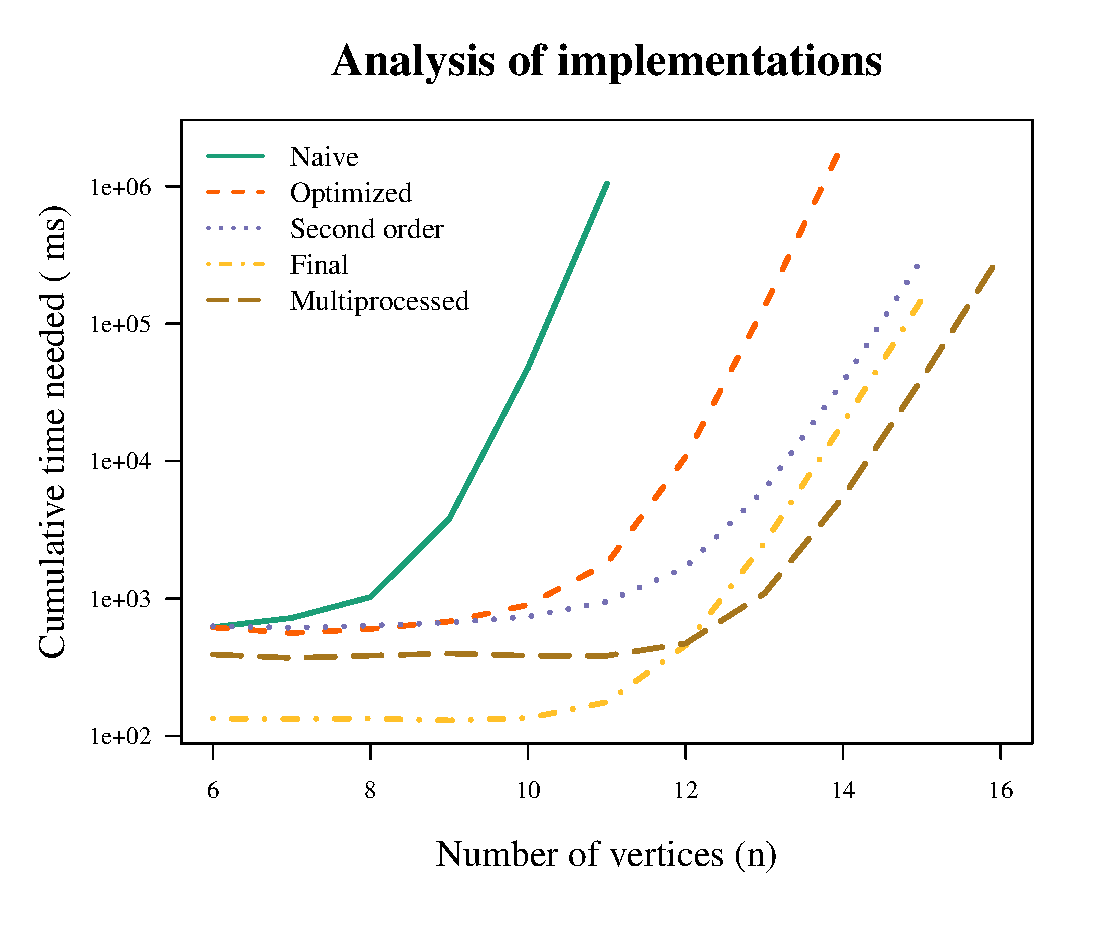
\includegraphics[width=0.45\textwidth]{figures/General_comparison.pdf}
	\caption{A comparison between different versions of the algorithm, tested on all planar triangulations for a given number of vertices. \DIFdelbeginFL \DIFdelFL{The naive algorithm is the simplest algorithm described in Algorithm \ref{alg:naive}. Optimized is the implementation that has implemented the available colors, permutations and bit-sets optimizations. The second order implementation has also implemented the updating of neighbors' neighbors. Lastly, the final and multithreaded implementations are the final C implementation and its multithreaded version using 10 processes respectively. }\DIFdelendFL Each implementation performs better than the last.}\label{fig:general}
\end{figure}


\subsubsection{Data structures}

For the implementation of the algorithm, multiple data structures for monitoring vertices were tested.
These include a simple list of vertices, a priority queue and a bit-set implementation. \DIFaddbegin \DIFadd{These structures are all discussed because of some strengths each seemingly has. }\DIFaddend The speed of these data structures are tested against each other.

\DIFdelbegin \DIFdel{These structures are all considered because of some strengths each seemingly has. }\DIFdelend The list of vertices is \DIFdelbegin \DIFdel{very simple , and }\DIFdelend \DIFaddbegin \DIFadd{a simple data structure, as the updating of a vertex does not demand a change of order in the list. It }\DIFaddend could therefore work well. The priority queue sorts the vertices by the amount of available colors (from low to high), and therefore has easy \DIFdelbegin \DIFdel{look-up }\DIFdelend \DIFaddbegin \DIFadd{lookup }\DIFaddend for the best vertex to color\DIFdelbegin \DIFdel{in}\DIFdelend . And lastly, the bit-set data structure, implemented using a list of bit-sets, where each index of the list denotes a number of available colors. The bit-sets then indicate if a vertex either has or \DIFdelbegin \DIFdel{doesn't }\DIFdelend \DIFaddbegin \DIFadd{does not }\DIFaddend have a certain amount of available colors. \DIFaddbegin \DIFadd{The last two structures allow the algorithm to find the next optimal vertex to color in constant time, while the list can only do this in worst-case linear time.
}\DIFaddend 

The comparison between \DIFdelbegin \DIFdel{datastructures }\DIFdelend \DIFaddbegin \DIFadd{data structures }\DIFaddend is found in Figure \ref{fig:datastruct}. It is clear the priority queue method performs the worst. This is because updating the number of available colors requires a completely new entry in the queue, which \DIFdelbegin \DIFdel{has }\DIFdelend \DIFaddbegin \DIFadd{causes }\DIFaddend too much overhead. Both the bit-set and standard list implementation perform almost equally well in the figure. \DIFdelbegin \DIFdel{Since }\DIFdelend \DIFaddbegin \DIFadd{But since }\DIFaddend the scale of the y-axis in the figure is logarithmic, the difference is still substantial. 
\DIFdelbegin \DIFdel{Therefore, going }\DIFdelend \DIFaddbegin 

\DIFadd{This difference is caused by the small overhead the bit-set data structure has in updating the state of a vertex. Whenever the number of available colors changes, the position of that vertex in the data structure should change. The easy lookup for the next vertex to color does not counteract this slow-down enough for bit-sets to perform better than a simple list.
}

\DIFadd{Going }\DIFaddend forward, the \DIFdelbegin \DIFdel{simple list datastructure }\DIFdelend \DIFaddbegin \DIFadd{list data structure }\DIFaddend is used.

\begin{figure}
	\centering
	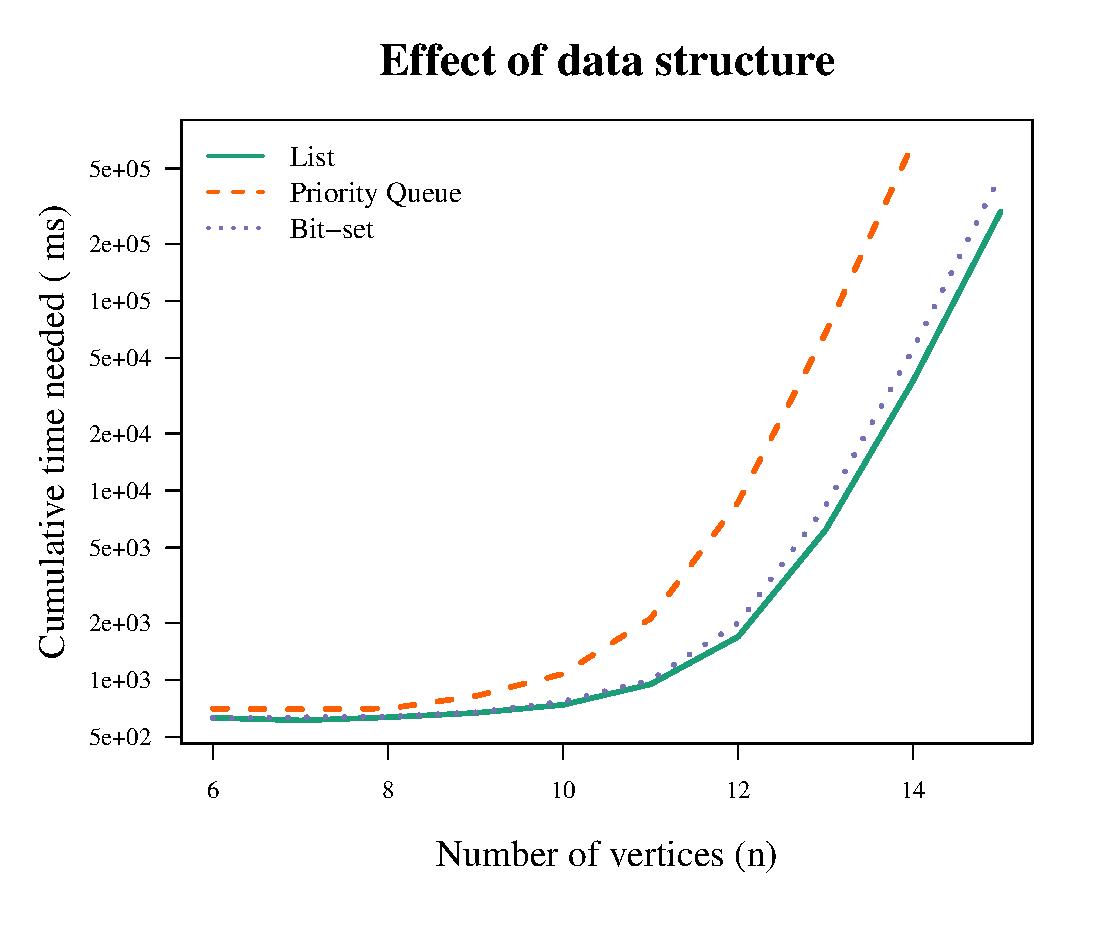
\includegraphics[width=0.45\textwidth]{figures/Datastructures_comparison.pdf}
	\caption{A comparison between the discussed datastructures. The simple list structure performs the best.}\label{fig:datastruct}
\end{figure}

\subsubsection{Index}

In total, \DIFdelbegin \DIFdel{three }\DIFdelend \DIFaddbegin \DIFadd{five }\DIFaddend different \texttt{get\_best\_index}-techniques were tested\DIFdelbegin \DIFdel{out}\DIFdelend . These techniques \DIFdelbegin \DIFdel{ranged }\DIFdelend \DIFaddbegin \DIFadd{range }\DIFaddend from simply finding the vertex with the least amount of available colors, to finding the vertex with the highest degree. Some methods were adapted from results found by Aslan and Baykan \cite{aslan2016performance}. \DIFdelbegin \DIFdel{Of these $5$, the }\DIFdelend \DIFaddbegin \DIFadd{Only the three }\DIFaddend best-performing \DIFdelbegin \DIFdel{and simplest }\DIFdelend methods are compared \DIFdelbegin \DIFdel{.
}%DIFDELCMD < 

%DIFDELCMD < %%%
\DIFdel{These include the two previously-mentioned methods, respectively called Standard and Welsh Powell (WP), are compared against Standard\_WP: a combination of the two techniques, using the standard technique with a degree tiebreaker}\DIFdelend \DIFaddbegin \DIFadd{here}\DIFaddend .

Other \DIFaddbegin \DIFadd{worse }\DIFaddend methods mentioned by Aslan and Baykan, such as DSATUR and First Fit either had overhead in registering extra data specifically for the technique, or were too simple and thus \DIFaddbegin \DIFadd{already }\DIFaddend performed badly in the original paper. Therefore, these are not considered \DIFaddbegin \DIFadd{in the comparison.
}

\DIFadd{The three best techniques include the two methods mentioned earlier (least number of available colors and highest degree), respectively named Standard and Welsh Powell (WP), and a Standard\_WP-method, a combination of the two: using the Standard technique with a degree tiebreaker}\DIFaddend . 

Figure \ref{fig:index} shows the comparison of \DIFdelbegin \DIFdel{the three discussed }\DIFdelend \DIFaddbegin \DIFadd{these }\DIFaddend techniques. Here, there is no doubt that the standard least amount of available colors performs best. It does look like \DIFdelbegin \DIFdel{both }\DIFdelend \DIFaddbegin \DIFadd{all }\DIFaddend curves grow as fast for the number of vertices, but the growth phase of the standard technique starts later. Therefore, this index-choosing technique is used from here on out. 

\begin{figure}
	\centering
	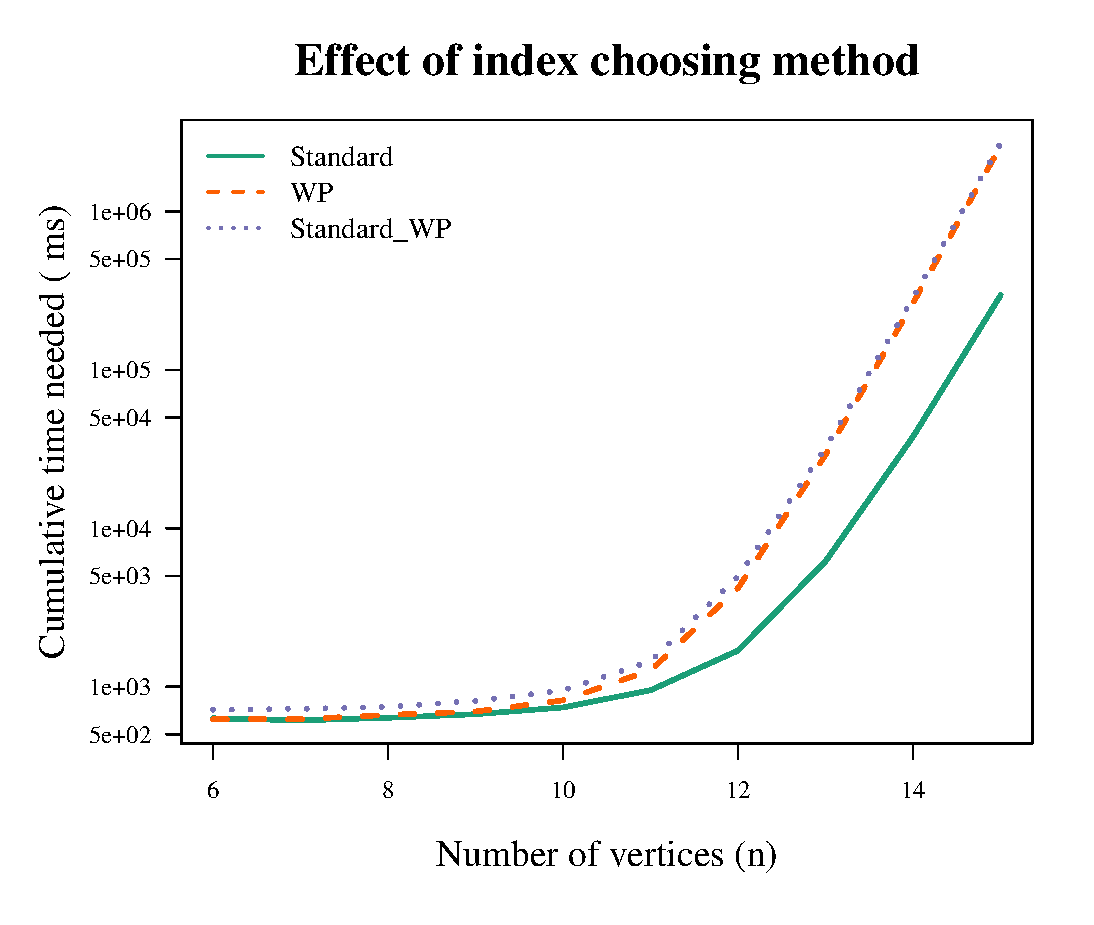
\includegraphics[width=0.45\textwidth]{figures/Index_comparison.pdf}
	\caption{The choosing of next vertex indices is compared for \DIFdelbeginFL \DIFdelFL{$3$ }\DIFdelendFL \DIFaddbeginFL \DIFaddFL{three }\DIFaddendFL methods. WP and Standard\_WP perform almost equal. The standard method grows the slowest.}\label{fig:index}
\end{figure}


\subsubsection{Second order optimization}
\label{sec:secondorder}

Instead of only updating the available colors of vertices' neighbors, those of the neighbors' neighbors can also change when coloring a vertex. Here, this is only done when there is only one uncolored vertex left in the neighborhood of the neighbor. One of those rules is displayed in Algorithm \ref{alg:special} for the odd coloring. As mentioned before, the other colorings also have similar rules.

The rule for the unique-maximum coloring checks the number of times the maximum color occurs, if this is only once, prohibit the use of that color, otherwise, the uncolored vertex needs an even higher color to create a new maximum color.

The conflict-free rule checks whether any colors occur once, if not, the uncolored vertex should get a unique color. Otherwise, if there is only one color occurring once, this color should get avoided, if there are multiple, nothing happens. 

The effect of using these second-order optimizations is visible in Figure \ref{fig:general}. This optimization clearly makes the algorithm perform better. It even results in a slower growth of \DIFdelbegin \DIFdel{needed }\DIFdelend \DIFaddbegin \DIFadd{execution }\DIFaddend time.

\subsubsection{Parallelization}

A simple but effective optimization to apply is the use of parallelization. By using the already \DIFdelbegin \DIFdel{defined }\DIFdelend \DIFaddbegin \DIFadd{provided }\DIFaddend $RES/MOD$ option in \textit{plantri}\DIFdelbegin \DIFdel{, an }\DIFdelend \DIFaddbegin \DIFadd{---an }\DIFaddend option to split up the generated graphs into disjoint \DIFdelbegin \DIFdel{sets, the coloring of the }\DIFdelend \DIFaddbegin \DIFadd{sets---the coloring of }\DIFaddend graphs is easily done using multiprocessing\DIFdelbegin \DIFdel{. A }\DIFdelend \DIFaddbegin \DIFadd{: a }\DIFaddend procedure where a new process is created for each of \DIFdelbegin \DIFdel{the }\DIFdelend \DIFaddbegin \DIFadd{those }\DIFaddend independent sets generated. This allows for a significant speedup dependent on the architecture of the system used (\textit{i.e., number of cores})\DIFdelbegin \DIFdel{. Because now more of the cores }\DIFdelend \DIFaddbegin \DIFadd{, because now more resources }\DIFaddend of the CPU \DIFdelbegin \DIFdel{are used, instead of only one}\DIFdelend \DIFaddbegin \DIFadd{can be used}\DIFaddend .
All outputs are then generated in different output files and combined at finish time.

A comparison between the normal and multiprocessed implementations \DIFaddbegin \DIFadd{(run using $10$ processes) }\DIFaddend is shown in Figure \ref{fig:general}. As expected, for less graphs, splitting up all graphs \DIFdelbegin \DIFdel{, }\DIFdelend and combining the results will take longer than \DIFdelbegin \DIFdel{only }\DIFdelend \DIFaddbegin \DIFadd{simply }\DIFaddend coloring the graphs. \DIFdelbegin \DIFdel{After planar triangulations with }\DIFdelend \DIFaddbegin \DIFadd{For graphs with more than }\DIFaddend $12$ vertices, the speedup of using multiprocessing does become apparent. 

\subsubsection{Porting to C}

The last optimization is the moving of the \DIFdelbegin \DIFdel{code }\DIFdelend \DIFaddbegin \DIFadd{implementation }\DIFaddend from Java to C\DIFdelbegin \DIFdel{, a low-level programming language}\DIFdelend . The difference between \DIFdelbegin \DIFdel{the two languages is }\DIFdelend \DIFaddbegin \DIFadd{these two languages lies }\DIFaddend in the extra overhead found in Java\DIFdelbegin \DIFdel{. Java }\DIFdelend \DIFaddbegin \DIFadd{, which }\DIFaddend uses features like a garbage collector to monitor memory usage. C does not, which allows it to process graphs faster, but it does call for a more careful approach.

Only the best-performing \DIFdelbegin \DIFdel{datastructures }\DIFdelend \DIFaddbegin \DIFadd{data structures }\DIFaddend and optimizations are added in C. These \DIFdelbegin \DIFdel{will therefore not be }\DIFdelend \DIFaddbegin \DIFadd{are therefore not }\DIFaddend compared again in C.

Figure \ref{fig:general} shows a comparison between the Java second order implementation and the Final C implementation. The final version does have \DIFaddbegin \DIFadd{some }\DIFaddend extra smaller optimizations, but even comparing both on \DIFdelbegin \DIFdel{almost }\DIFdelend the exact same implementation \DIFdelbegin \DIFdel{still favours C}\DIFdelend \DIFaddbegin \DIFadd{will still favor C, as is expected}\DIFaddend .


\subsection{Correctness}
\label{sec:correctness}

The correctness of the \DIFdelbegin \DIFdel{implemented }\DIFdelend \DIFaddbegin \DIFadd{final }\DIFaddend algorithm is never guaranteed. This is different for very simple versions of the algorithm. By comparing a naive implementation to the final implementation in C, discrepancies in coloring results can get found and resolved. 

% naive
\begin{algorithm}[tb]
	\caption{\texttt{can\_color\_with\_max\_c\_naive}}
	\label{alg:naive}
	\textbf{Parameters}: The graph $G$, coloring $K$, max. color $max\_c$ and $index$ \\
	\textbf{Output}: Coloring achieved
	\begin{algorithmic}[1]
		\IF{$index \ge G.nb\_vertices$}

		\RETURN \texttt{is\_correctly\_colored}($G, K$)
		\ENDIF

		\FOR{$c$ { from} $1$ {to} $max\_c$}

		\STATE $G.vertices$[$index$]$.color \gets c$

		\IF{\texttt{can\_color\_with\_max\_c\_naive}($G, K, max\_c, index$)}

		\RETURN true

		\ENDIF

		\ENDFOR

		\RETURN false
	\end{algorithmic}
\end{algorithm}

The naive algorithm is displayed in Algorithm \ref{alg:naive}. The code reflects the \DIFdelbegin \DIFdel{pseudo-code }\DIFdelend \DIFaddbegin \DIFadd{pseudocode }\DIFaddend almost one-to-one. Therefore, it is clear that the naive implementation functions by testing every possible coloring given a maximum color. \DIFdelbegin \DIFdel{This }\DIFdelend \DIFaddbegin \DIFadd{The naive }\DIFaddend implementation can hence be considered \DIFaddbegin \DIFadd{(practically) }\DIFaddend correct.

\DIFdelbegin \DIFdel{All }\DIFdelend \DIFaddbegin \DIFadd{Correctness for all }\DIFaddend planar triangulations with number of vertices $4 \le n \le 12$ were tested for all coloring variants \DIFaddbegin \DIFadd{by comparing the final and naive implementations. The improper colorings (}\textit{\DIFadd{e.g., $\mathrm{iUMc}$}}\DIFadd{) have lower chromatic numbers overall, therefore these were tested to a maximum of $14$ vertices}\DIFaddend .
For the proper coloring, an extra tool called \textit{nauty}\DIFaddbegin \DIFadd{, }\DIFaddend developed by McKay and Piperno, is used \cite{mckay2014practical}. This tool can find the chromatic numbers for any graph efficiently. Therefore, more planar triangulations \DIFdelbegin \DIFdel{were tested, }\DIFdelend \DIFaddbegin \DIFadd{could be tested: }\DIFaddend those with number of vertices $4 \le n \le 20$.
\DIFdelbegin \DIFdel{The improper colorings (}\textit{\DIFdel{e.g., $\mathrm{iUMc}$}}%DIFAUXCMD
\DIFdel{) have lower chromatic numbersoverall, therefore these were tested to a maximum of $14$ vertices. }\DIFdelend 


\DIFdelbegin \DIFdel{All tests found that }\DIFdelend \DIFaddbegin \DIFadd{These tests found correct output, meaning the exact same chromatic numbers, for the final implementation when compared to these more trusted implementations (}\textit{\DIFadd{nauty}} \DIFadd{and naive implementation). This gives us high confidence in the correctness of }\DIFaddend the final implementation\DIFdelbegin \DIFdel{works correctly}\DIFdelend .

\section{Results}
\label{sec:results}

Now that the researched problem and the developed algorithm have been discussed, the research questions are revisited. 

The only coloring variant for which any widespread algorithms exist, is the proper coloring. As mentioned before, this includes tools like \textit{nauty}. No \DIFdelbegin \DIFdel{open-source }\DIFdelend \DIFaddbegin \DIFadd{open source }\DIFaddend coloring tool for \DIFaddbegin \DIFadd{any of }\DIFaddend the other colorings exists. This means a comparison for efficiency for all coloring variants \DIFdelbegin \DIFdel{will not be }\DIFdelend \DIFaddbegin \DIFadd{is not }\DIFaddend possible.

Comparing \textit{nauty}'s coloring option against the developed algorithm has expected results. As seen in Table \ref{tab:nauty}, \textit{nauty} is faster in coloring all planar triangulations with some number of vertices. It can be noted that the program developed here is still performing well. Around $1.4$ times slower than \textit{nauty}. For higher number of vertices, the ratio between the two \DIFdelbegin \DIFdel{is getting }\DIFdelend \DIFaddbegin \DIFadd{does get }\DIFaddend smaller, indicating the developed algorithm may \DIFdelbegin \DIFdel{become }\DIFdelend \DIFaddbegin \DIFadd{be }\DIFaddend better for graphs with a high number of vertices.


\begin{table}
	\centering
	\begin{tabular}{r|ll|r} 
		\hline
		Number of vertices & This program ($s$) & \textit{Nauty} ($s$) & Ratio \\
		\hline
		$10$ & $0.013$ & $0.003$ & $4.3$ \\ 
		$11$ & $0.014$ & $0.004$ & $3.5$ \\
		$12$ & $0.020$ & $0.008$ & $2.5$ \\
		$13$ & $0.064$ & $0.039$ & $1.64$ \\
		$14$ & $0.39$ & $0.25$ & $1.56$ \\
		$15$ & $2.9$ & $1.9$ & $1.54$ \\
		$16$ & $22$ & $15$ & $1.49$ \\
		$17$ & $177$ & $121$ & $1.46$ \\
		$18$ & $1.4 \times 10^{3}$ & $1.0 \times 10^{3}$ & $1.41$
	\end{tabular}
	\caption{A comparison between the program developed in this paper and \textit{nauty}. Compared for all planar triangulations with a given number of vertices. \textit{Nauty} outperforms this program for all number of vertices. The ratio between the two tools goes down for more number of vertices.}\label{tab:nauty}
\end{table}


\textit{Nauty} is specifically designed for \DIFdelbegin \DIFdel{the }\DIFdelend coloring with the proper coloring. The other coloring variants discussed are not supported. These would also require the addition of completely new functions, and a lot of code duplication; or a complete rework of the algorithm. Therefore, \textit{nauty} can not be easily expanded to new colorings, such as those discussed here, whereas this is possible for \DIFdelbegin \DIFdel{the }\DIFdelend \DIFaddbegin \DIFadd{our }\DIFaddend developed algorithm. All coloring-dependent methods can be easily expanded without much added work. 
\DIFdelbegin \DIFdel{Additionally, }\textit{\DIFdel{nauty}} %DIFAUXCMD
\DIFdel{does not automatically support the use of multiprocessing, while this is supported for our implementation. 
}\DIFdelend 

The other colorings are not comparable to other tools. Therefore, profiling the speed or efficiency of the algorithm is hard. But \DIFdelbegin \DIFdel{it does compare }\DIFdelend \DIFaddbegin \DIFadd{since it compares }\DIFaddend quite well to \textit{nauty}, and is also very expandable, \DIFdelbegin \DIFdel{which does mean it is efficient in that sense}\DIFdelend \DIFaddbegin \DIFadd{it does allow us to conclude the algorithm is rather efficient}\DIFaddend .


The second research question concerned the use of the algorithm for disproving or substantiating conjectures. This is an exhaustive algorithm, therefore, all possible graphs for a given number of graphs can be checked to see if they follow a conjecture or not.

Here, all planar triangulations---graphs with the highest possible number of edges\DIFdelbegin \DIFdel{and therefore graphs with }\DIFdelend \DIFaddbegin \DIFadd{, which therefore have }\DIFaddend a higher average chromatic number---with $n$ vertices were checked ($4 \le n \le 20$). It was \DIFdelbegin \DIFdel{found }\DIFdelend \DIFaddbegin \DIFadd{determined }\DIFaddend that these graphs all conform to the current conjectures on chromatic numbers for all \DIFdelbegin \DIFdel{colorings}\DIFdelend \DIFaddbegin \DIFadd{coloring variants. Since planar triangulations are only a subset of all planar graphs, it could still mean there are planar graphs with a higher chromatic number for the same number of vertices $n$ (}\textit{\DIFadd{e.g., the smallest graph with a chromatic number of $4$ for the $\mathrm{iCFo}$-coloring is not a planar triangulation}}\DIFadd{). 
}

\DIFadd{Still, only planar triangulations are checked here because the amount of planar graphs grows substantially faster than the number of planar triangulations. There are more planar graphs with only $13$ vertices than planar triangulations with $20$ vertices}\DIFaddend . 

The program can also assist in disproving the conjectures. An option \DIFaddbegin \DIFadd{for the program }\DIFaddend is provided that will check all possible colorings of a given graph. This allows the user to assert if a graph has a certain property, helping in the search for \DIFdelbegin \DIFdel{gadgets---graphs }\DIFdelend \DIFaddbegin \DIFadd{gadgets: graphs }\DIFaddend which help in the disproving or proving of some theorem or conjecture. 

The unique-maximum \DIFdelbegin \DIFdel{colorings have a }\DIFdelend \DIFaddbegin \DIFadd{coloring variants have a interesting }\DIFaddend property useful in the finding of gadgets, which the program can search for. As visible in Figure \ref{fig:graph}, there exist graphs with vertices that always have a certain color. These are great examples of gadgets, findable by the program. This is only applicable to the unique-maximum coloring variants, because as said before, permutations of other coloring variants still lead to a valid coloring. Therefore, for these other variants, no vertex can always have the same color. \DIFaddbegin \DIFadd{But, other properties for these colorings are still possible.
}\DIFaddend 

\begin{figure}
	\begin{center}
		\DIFdelbeginFL %DIFDELCMD < \begin{tikzpicture}[
%DIFDELCMD < 			% Define the style for the nodes
%DIFDELCMD < 			every node/.style={circle, draw, thick, minimum size=5mm}
%DIFDELCMD < 			]
%DIFDELCMD < 			

%DIFDELCMD < 			\node (v1) at (0, 0) [fill=orange]  {2};
%DIFDELCMD < 			\node (v2) at (0, 6) [fill=blue!50] {1};
%DIFDELCMD < 			\node (v3) at (-3, 3) [fill=blue!50]{1};
%DIFDELCMD < 			\node (v4) at (3, 3) [fill=blue!50]{1};
%DIFDELCMD < 			\node (v5) at (0, 3) [fill=green!80]{3};
%DIFDELCMD < 			

%DIFDELCMD < 			\draw[thick] (v1)--(v3);
%DIFDELCMD < 			\draw[thick] (v1)--(v4);
%DIFDELCMD < 			

%DIFDELCMD < 			\draw[thick] (v5)--(v1);
%DIFDELCMD < 			\draw[thick] (v5)--(v2);
%DIFDELCMD < 			\draw[thick] (v5)--(v3);
%DIFDELCMD < 			\draw[thick] (v5)--(v4);
%DIFDELCMD < 			

%DIFDELCMD < 		\end{tikzpicture}
%DIFDELCMD < 	%%%
\DIFdelendFL \DIFaddbeginFL 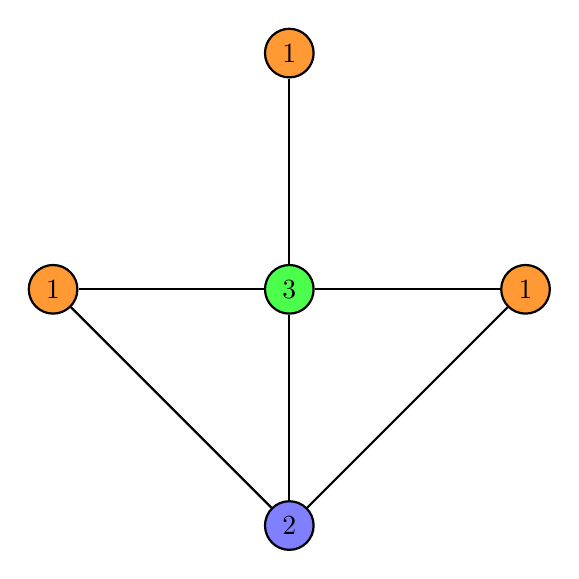
\begin{tikzpicture}[
			% Define the style for the nodes
			every node/.style={circle, draw, thick, minimum size=5mm}
			]

			\node (v1) at (0, 0) [fill=blue!50]  {2};
			\node (v2) at (0, 6) [fill=orange!80] {1};
			\node (v3) at (-3, 3) [fill=orange!80]{1};
			\node (v4) at (3, 3) [fill=orange!80]{1};
			\node (v5) at (0, 3) [fill=green!70]{3};

			\draw[thick] (v1)--(v3);
			\draw[thick] (v1)--(v4);

			\draw[thick] (v5)--(v1);
			\draw[thick] (v5)--(v2);
			\draw[thick] (v5)--(v3);
			\draw[thick] (v5)--(v4);

		\end{tikzpicture}
	\DIFaddendFL \end{center}
	\caption{A colored graph for the $\mathrm{pUMo}$ coloring, where each vertex with color $1$ can only have that color. Giving it any other color would result in an invalid coloring.}\label{fig:graph}
\end{figure}


\section{Threats to validity}
\label{sec:threats}

As explained in Section \ref{sec:correctness}, the correctness of the implementation is never guaranteed. Furthermore, the comparison between implementations also \DIFdelbegin \DIFdel{doesn't }\DIFdelend \DIFaddbegin \DIFadd{does not }\DIFaddend guarantee correctness for graphs that were never tested, such as graphs with a high number of vertices. 
There is still a possibility that the naive implementation \DIFdelbegin \DIFdel{isn't }\DIFdelend \DIFaddbegin \DIFadd{is not }\DIFaddend implemented correctly. However, this is unlikely because of the perfect reflection between implementation and algorithm. Still, the \texttt{is\_correctly\_colored}-check, seen in Algorithm \ref{alg:naive}, could function incorrectly.

The output of the proper coloring was tested against \textit{nauty}. There is no guarantee of the correctness of \textit{nauty}'s implementation.

All optimization experiments were performed on one specific machine, other computer architectures could yield a different outcome. 
Additionally, comparison of implementation decisions---the optimizations presented---are only tested at one implementation stage (\textit{e.g., naive implementation, post-bit-set implementation}), all tested in Java, and not at each stage of implementation. This could mean that some optimizations applied to the final program may result in different observations. For example, results of optimizations could differ when implemented in C.

\section{Conclusion}
\label{sec:conclusion}

In conclusion, this paper discussed a computational approach for the coloring of graphs. This is done for different variants of vertex colorings: \DIFdelbegin \DIFdel{namely }\DIFdelend the proper, odd, conflict-free and unique-maximum colorings. 

A backtracking algorithm for coloring planar graphs with these coloring variants is discussed. Firstly, the algorithm was developed in Java, to then be ported over to C for efficiency. In Java, multiple optimizations were tested out and implemented. Different data structures were considered, a simple list performing the best. Additionally, other optimizations such as the usage of bit-sets or parallelization were also considered. 
All optimizations were tested to ensure the optimality of the algorithm.

The correctness of the algorithm was checked by comparing the outputs from the final program to those of a naive version. The \DIFdelbegin \DIFdel{simpleness }\DIFdelend \DIFaddbegin \DIFadd{simplicity }\DIFaddend of the naive algorithm \DIFdelbegin \DIFdel{and its structure showed the correctness, }\DIFdelend combined with identical outputs \DIFdelbegin \DIFdel{, lets us accept the final algorithm as correct}\DIFdelend \DIFaddbegin \DIFadd{between the naive algorithm and the final implementation gives us very high confidence in the correctness of the developed program}\DIFaddend .


This algorithm is the first of its kind, allowing the coloring of graphs for many different variants as one open-source program. It allows users to quickly color in graphs for many different variants, useful in applications such as wireless networks and more.
The program \DIFdelbegin \DIFdel{isn't }\DIFdelend \DIFaddbegin \DIFadd{is not }\DIFaddend as fast as other coloring tools such as \textit{nauty} for the proper coloring. But the \DIFdelbegin \DIFdel{expandability and easy internal usage of parallelization, things }\DIFdelend \DIFaddbegin \DIFadd{easy expandability, something }\DIFaddend \textit{nauty} lacks, partly \DIFdelbegin \DIFdel{make }\DIFdelend \DIFaddbegin \DIFadd{makes }\DIFaddend up for this drawback. 

The conjectures surrounding the chromatic numbers for these colorings were examined further. It was found that the conjectures hold for all planar triangulations with less than or equal to $20$ vertices. This gives some indication that these could hold for more graphs, since planar triangulations---in general---have a higher \DIFdelbegin \DIFdel{the }\DIFdelend chromatic number. 


\subsection{Future work}

Future work could include the addition of more coloring variants into the program. This would allow the tool to be used for a wide range of problems. 
Additionally, other versions such as edge-, or face colorings could be included as well.

Next, the algorithm can be more optimized. For example multithreading when coloring one graph with a high number of vertices could speed up the program even further. Furthermore, other coloring rules, such as those described in Section \ref{sec:secondorder}, can be developed.

Lastly, further research could \DIFdelbegin \DIFdel{further improve bounds of }\DIFdelend \DIFaddbegin \DIFadd{include improving the bounds of the }\DIFaddend chromatic numbers for the discussed coloring variants. 


\section*{Use of genAI}

For this paper, generative AI was used for the creation of figures. Additionally, it was also used in helping the writing process of the helper bash- and python files used in the implementation (\textit{e.g., color.sh}).

%%%%%%%%%%%%%%%%%%%%%%%%%%%%%%%%%%%%%%%%%%%%


%% The file named.bst is a bibliography style file for BibTeX 0.99c
%\bibliographystyle{named}
\DIFdelbegin %DIFDELCMD < \bibliographystyle{unsrt}
%DIFDELCMD < %%%
\DIFdelend \DIFaddbegin \bibliographystyle{plain}
\DIFaddend %\bibliographystyle{amsplain}
\bibliography{references}

	
\end{document}

